% Native editable composition from verified, unchanged IDE images.
\begin{figure}[htbp]
  \centering
  \sbox0{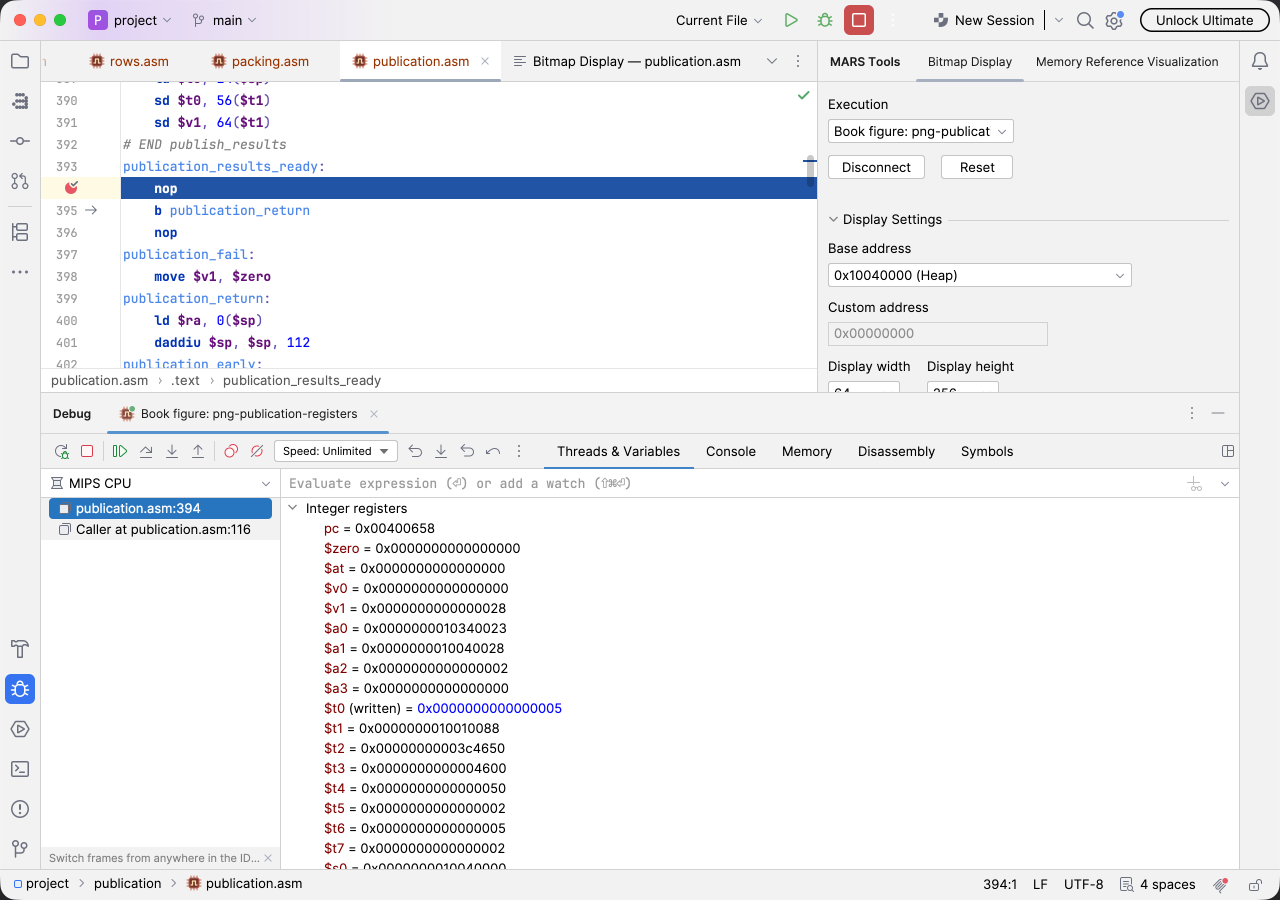
\includegraphics[artifact]{packages/033-png/captures/png-final-publication/registers.png}}
  \sbox2{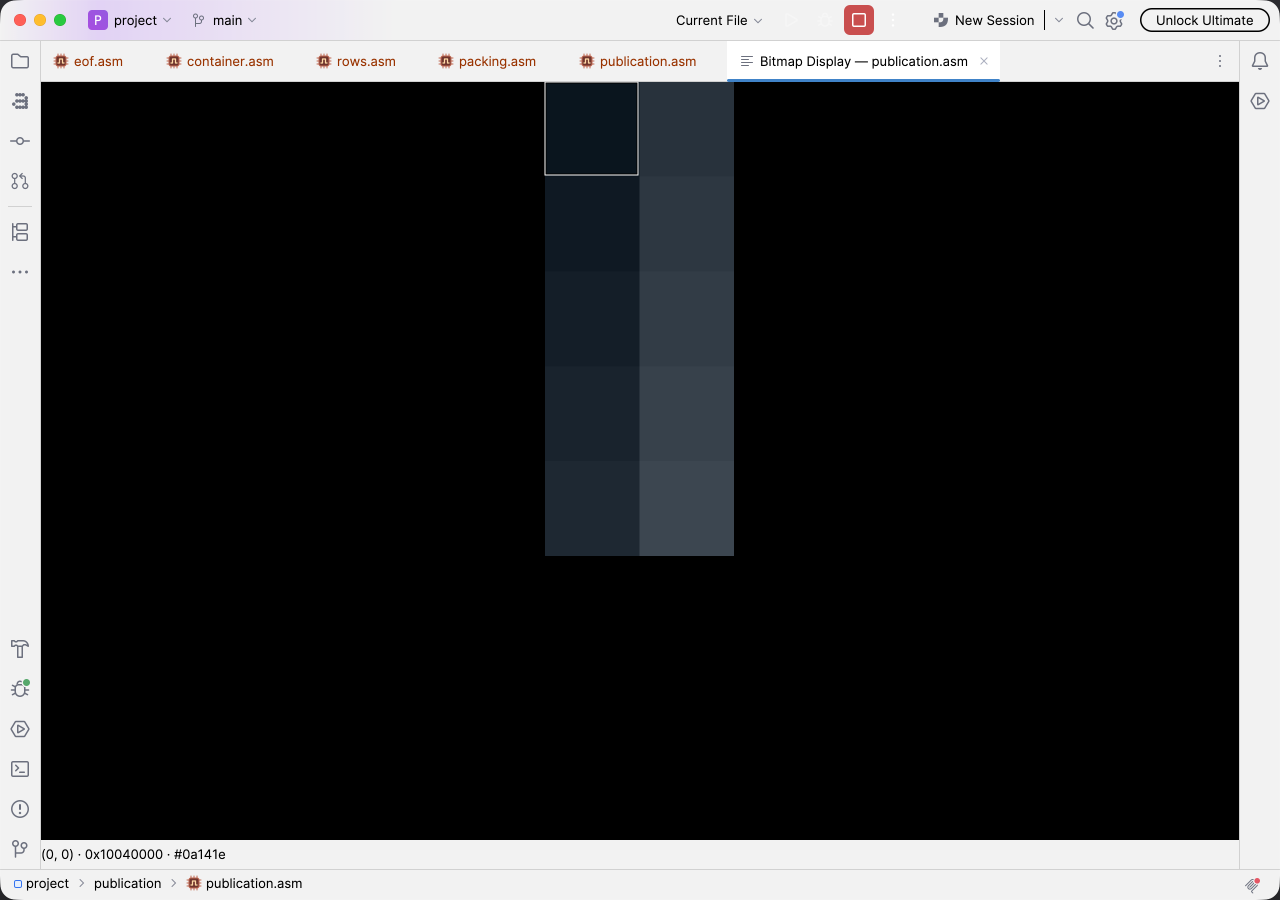
\includegraphics[artifact]{packages/033-png/captures/png-final-publication/bitmap.png}}
  \sbox4{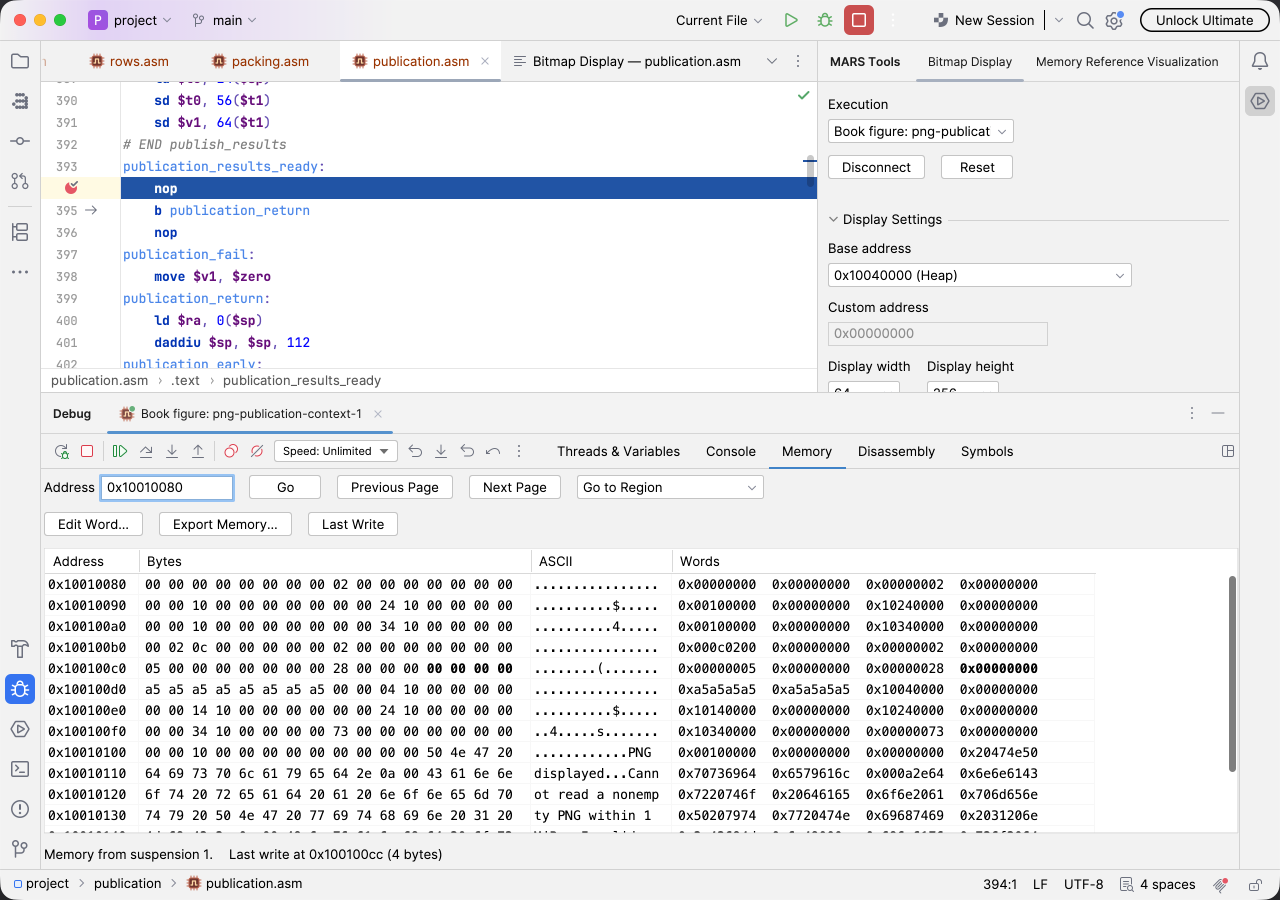
\includegraphics[artifact]{packages/033-png/captures/png-final-publication/context-1.png}}
  \sbox6{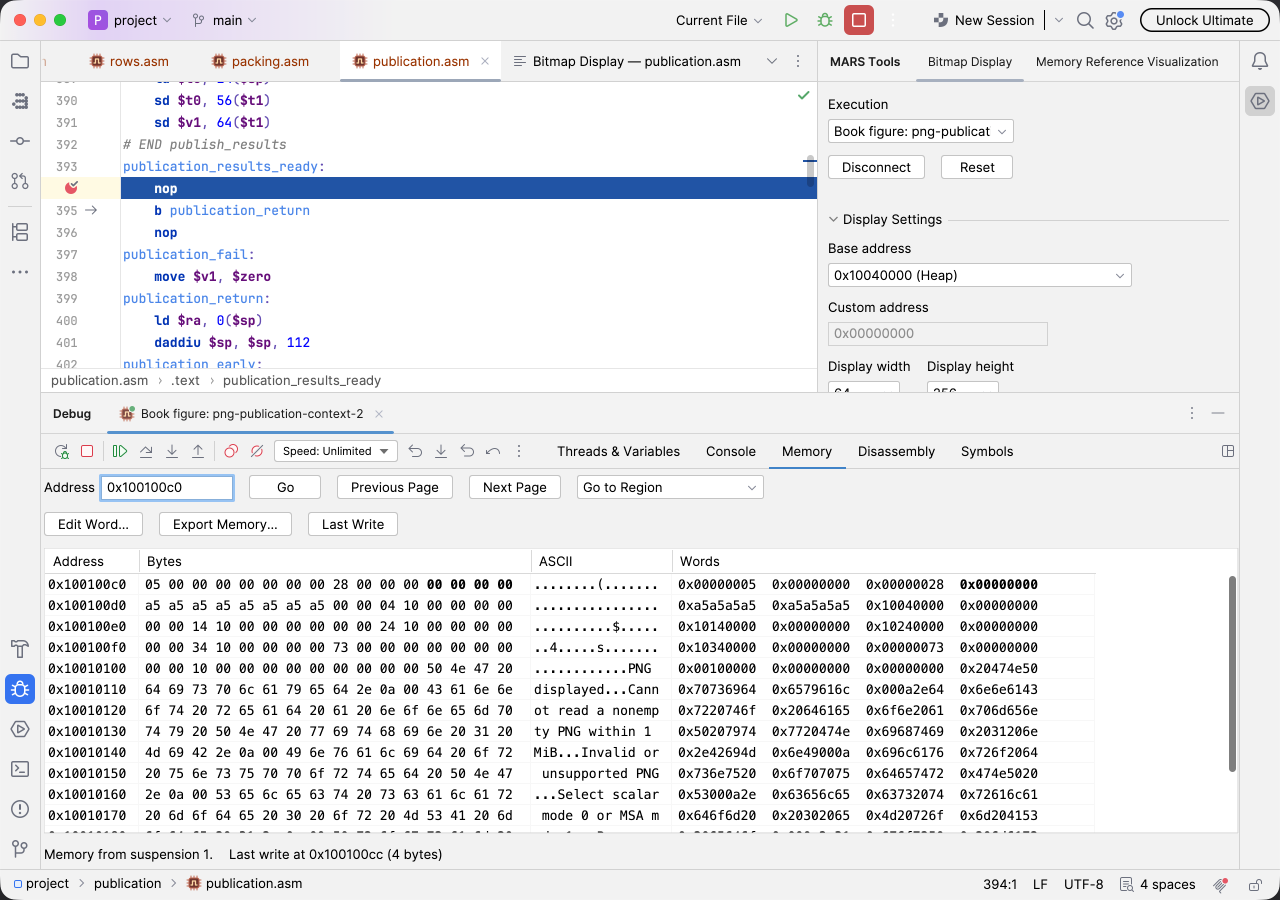
\includegraphics[artifact]{packages/033-png/captures/png-final-publication/context-2.png}}
  \edef\MARSpublicationsourceLeft{\the\dimexpr0.036718750\wd0\relax}
  \edef\MARSpublicationsourceBottom{\the\dimexpr0.774444444\ht0\relax}
  \edef\MARSpublicationsourceRight{\the\dimexpr0.611718750\wd0\relax}
  \edef\MARSpublicationsourceTop{\the\dimexpr0.170000000\ht0\relax}
  \edef\MARSpublicationbitmapLeft{\the\dimexpr0.421093750\wd2\relax}
  \edef\MARSpublicationbitmapBottom{\the\dimexpr0.066666667\ht2\relax}
  \edef\MARSpublicationbitmapRight{\the\dimexpr0.421875000\wd2\relax}
  \edef\MARSpublicationbitmapTop{\the\dimexpr0.091111111\ht2\relax}
  \edef\MARSpublicationdimensionsLeft{\the\dimexpr0.520312500\wd4\relax}
  \edef\MARSpublicationdimensionsBottom{\the\dimexpr0.265555556\ht4\relax}
  \edef\MARSpublicationdimensionsRight{\the\dimexpr0.139843750\wd4\relax}
  \edef\MARSpublicationdimensionsTop{\the\dimexpr0.704444444\ht4\relax}
  \edef\MARSpublicationcountLeft{\the\dimexpr0.520312500\wd6\relax}
  \edef\MARSpublicationcountBottom{\the\dimexpr0.312222222\ht6\relax}
  \edef\MARSpublicationcountRight{\the\dimexpr0.139843750\wd6\relax}
  \edef\MARSpublicationcountTop{\the\dimexpr0.634444444\ht6\relax}
  \edef\MARSpublicationreturnsLeft{\the\dimexpr0.246093750\wd0\relax}
  \edef\MARSpublicationreturnsBottom{\the\dimexpr0.310000000\ht0\relax}
  \edef\MARSpublicationreturnsRight{\the\dimexpr0.596875000\wd0\relax}
  \edef\MARSpublicationreturnsTop{\the\dimexpr0.638888889\ht0\relax}
  \begin{tikzpicture}[alt={Five annotated IDE details at publication_results_ready. The picture is two pixels wide and five rows high in a two-column eight-row display. The last three display rows are unused black rows. The first memory detail shows retained row capacity 786944 followed by published width two. The next detail shows published height five, forty active pixel bytes and the retained A5 suffix, followed by a pointer outside the context. Registers show success v0 zero and v1 forty. The compact recipe uses stride two pixels and retains the one MiB framebuffer allocation.}]
    \node[anchor=north west,inner sep=0,font=\small\bfseries] (source-title) at (6mm,0) {Final successful publication};
    \node[anchor=north west,inner sep=0] (source) at ([yshift=-1mm]source-title.south west) {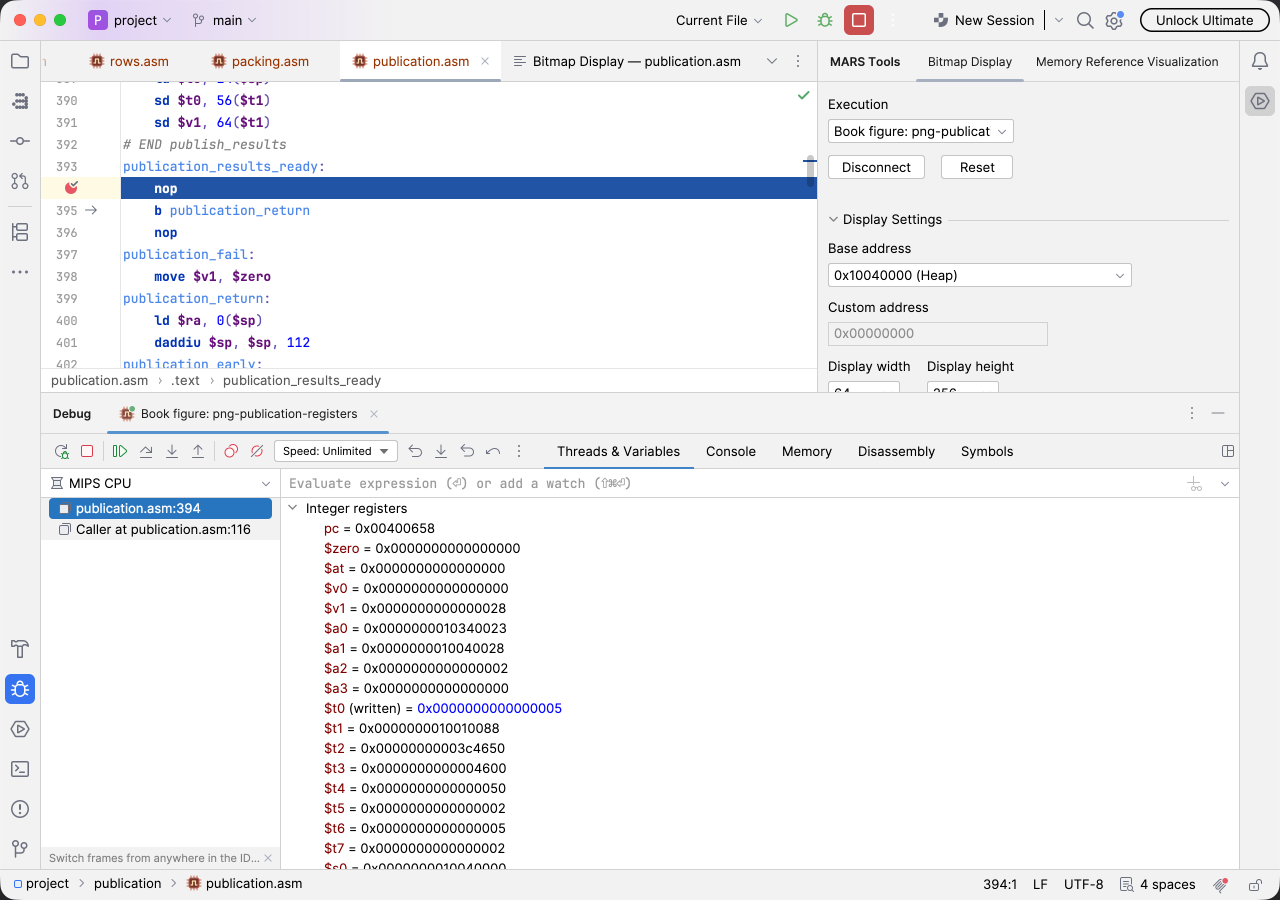
\includegraphics[width=0.7\linewidth,artifact,trim={\MARSpublicationsourceLeft{} \MARSpublicationsourceBottom{} \MARSpublicationsourceRight{} \MARSpublicationsourceTop{}},clip]{packages/033-png/captures/png-final-publication/registers.png}};
    \begin{scope}[shift={(source.south west)},x={($(source.south east)-(source.south west)$)},y={($(source.north west)-(source.south west)$)}]
      \draw[black,line width=0.7pt] (0.168888889,0.080000000) rectangle (0.288888889,0.520000000);
      \node[draw=black,fill=white,circle,inner sep=1.5pt,font=\footnotesize] at ($(0.168888889,0.520000000)+(-3mm,0)$) {1};
    \end{scope}
    \node[anchor=north west,inner sep=0,font=\small\bfseries] (bitmap-title) at ([yshift=-1.5mm]source.south west) {Five image rows, then three unused rows};
    \node[anchor=north west,inner sep=0] (bitmap) at ([yshift=-1mm]bitmap-title.south west) {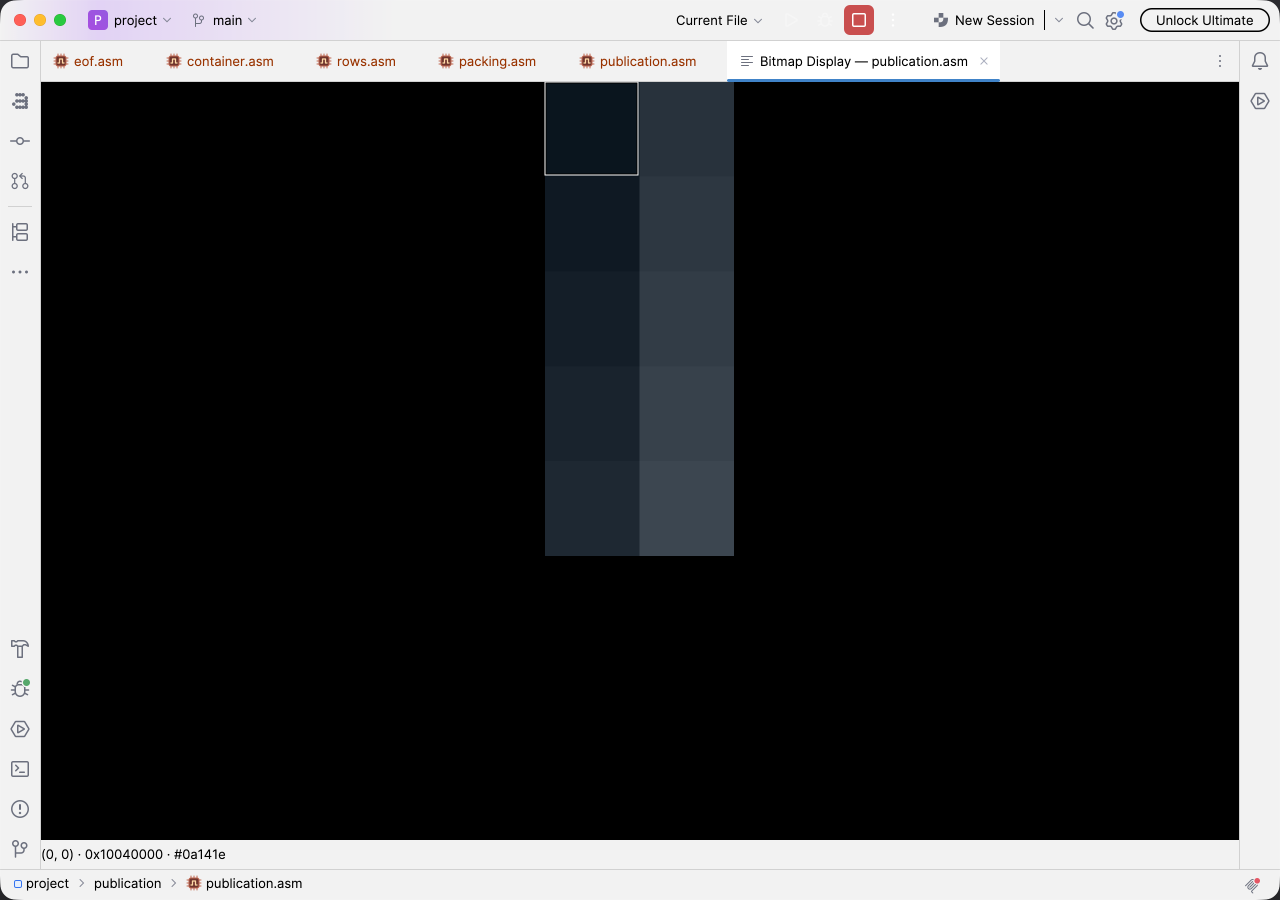
\includegraphics[width=0.08\linewidth,artifact,trim={\MARSpublicationbitmapLeft{} \MARSpublicationbitmapBottom{} \MARSpublicationbitmapRight{} \MARSpublicationbitmapTop{}},clip]{packages/033-png/captures/png-final-publication/bitmap.png}};
    \begin{scope}[shift={(bitmap.south west)},x={($(bitmap.south east)-(bitmap.south west)$)},y={($(bitmap.north west)-(bitmap.south west)$)}]
      \draw[black,line width=0.7pt] (0.029850746,0.000000000) rectangle (0.970149254,1.000000000);
      \node[draw=black,fill=white,circle,inner sep=1.5pt,font=\footnotesize] at ($(0.029850746,1.000000000)+(-3mm,0)$) {2};
    \end{scope}
    \node[anchor=north west,inner sep=0,font=\small\bfseries] (dimensions-title) at ([yshift=-1.5mm]bitmap.south west) {Retained row capacity and published width};
    \node[anchor=north west,inner sep=0] (dimensions) at ([yshift=-1mm]dimensions-title.south west) {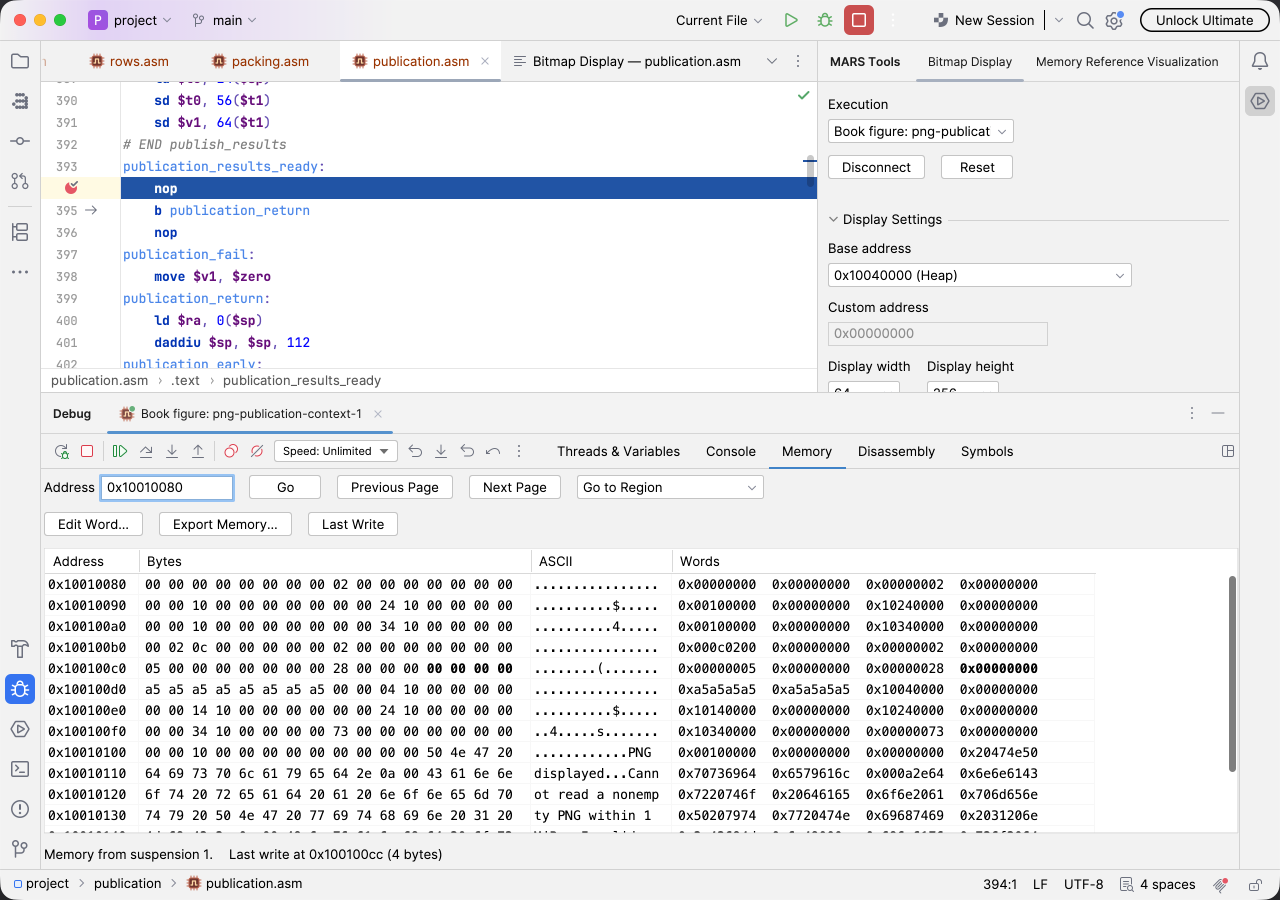
\includegraphics[width=0.84\linewidth,artifact,trim={\MARSpublicationdimensionsLeft{} \MARSpublicationdimensionsBottom{} \MARSpublicationdimensionsRight{} \MARSpublicationdimensionsTop{}},clip]{packages/033-png/captures/png-final-publication/context-1.png}};
    \begin{scope}[shift={(dimensions.south west)},x={($(dimensions.south east)-(dimensions.south west)$)},y={($(dimensions.north west)-(dimensions.south west)$)}]
      \draw[black,line width=0.7pt] (0.013793103,0.111111111) rectangle (0.986206897,0.888888889);
      \node[draw=black,fill=white,circle,inner sep=1.5pt,font=\footnotesize] at ($(0.013793103,0.888888889)+(-3mm,0)$) {3};
    \end{scope}
    \node[anchor=north west,inner sep=0,font=\small\bfseries] (count-title) at ([yshift=-1.5mm]dimensions.south west) {Height, active count and retained suffix};
    \node[anchor=north west,inner sep=0] (count) at ([yshift=-1mm]count-title.south west) {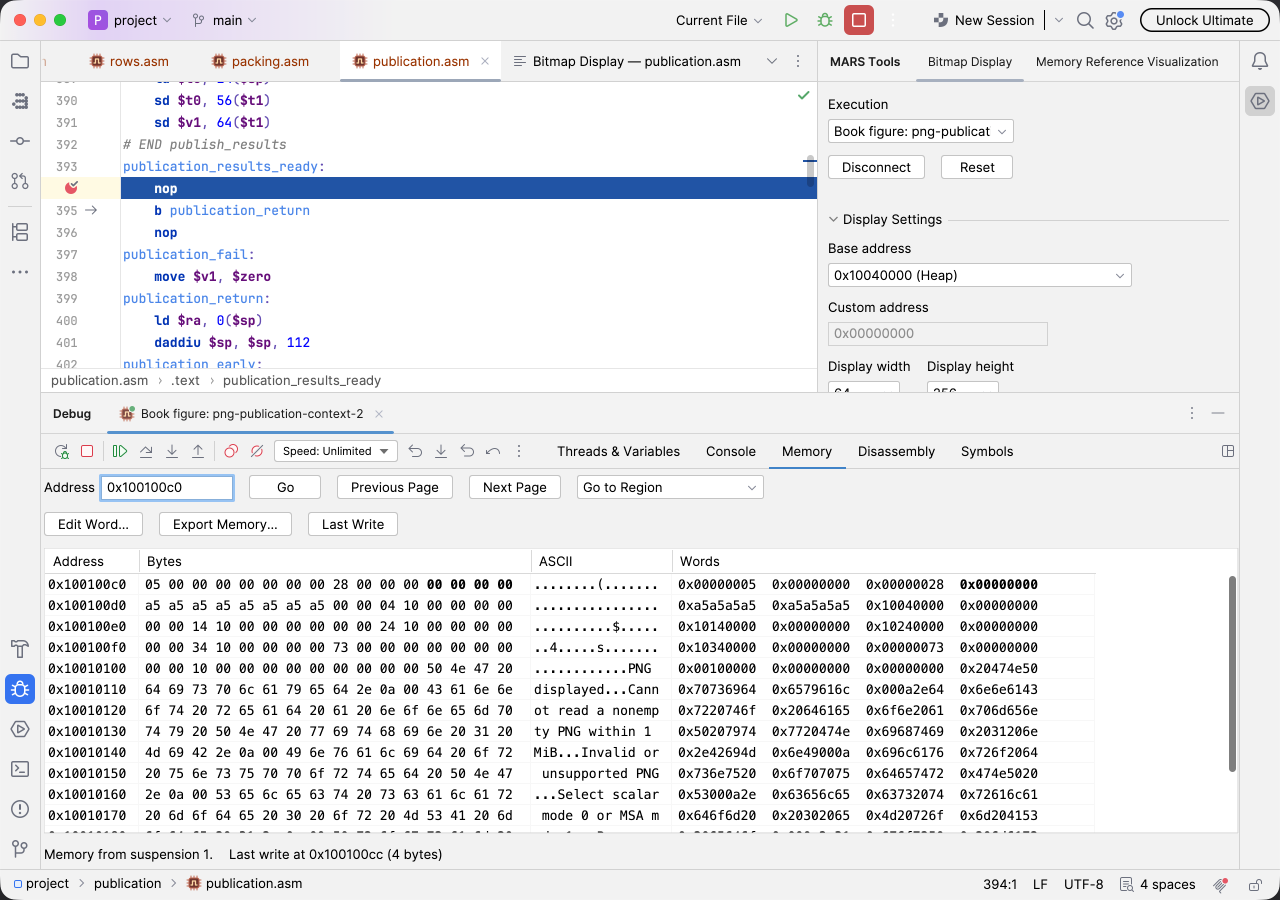
\includegraphics[width=0.84\linewidth,artifact,trim={\MARSpublicationcountLeft{} \MARSpublicationcountBottom{} \MARSpublicationcountRight{} \MARSpublicationcountTop{}},clip]{packages/033-png/captures/png-final-publication/context-2.png}};
    \begin{scope}[shift={(count.south west)},x={($(count.south east)-(count.south west)$)},y={($(count.north west)-(count.south west)$)}]
      \draw[black,line width=0.7pt] (0.013793103,0.062500000) rectangle (0.986206897,0.937500000);
      \node[draw=black,fill=white,circle,inner sep=1.5pt,font=\footnotesize] at ($(0.013793103,0.937500000)+(-3mm,0)$) {4};
    \end{scope}
    \node[anchor=north west,inner sep=0,font=\small\bfseries] (returns-title) at ([yshift=-1.5mm]count.south west) {Success and forty active bytes};
    \node[anchor=north west,inner sep=0] (returns) at ([yshift=-1mm]returns-title.south west) {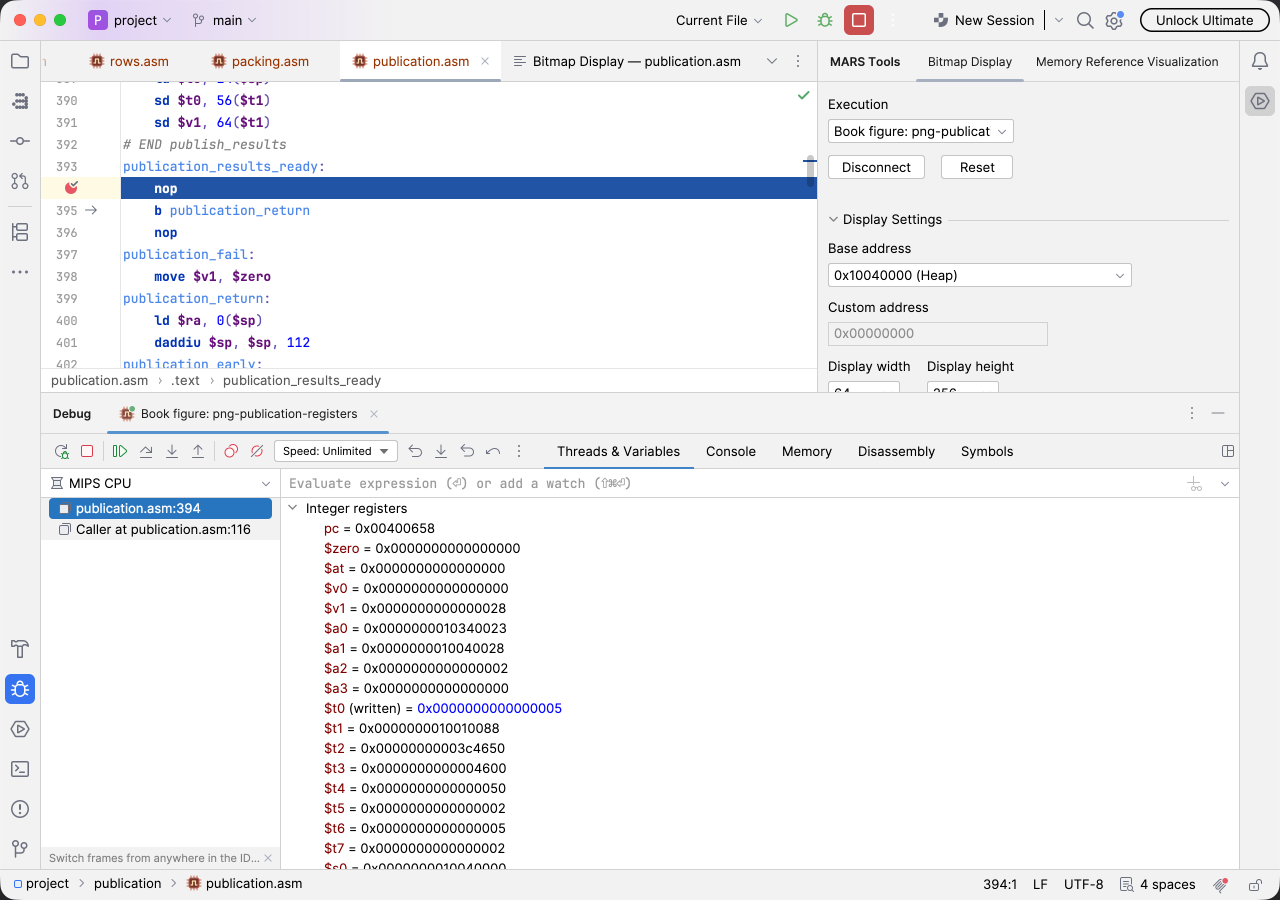
\includegraphics[width=0.5\linewidth,artifact,trim={\MARSpublicationreturnsLeft{} \MARSpublicationreturnsBottom{} \MARSpublicationreturnsRight{} \MARSpublicationreturnsTop{}},clip]{packages/033-png/captures/png-final-publication/registers.png}};
    \begin{scope}[shift={(returns.south west)},x={($(returns.south east)-(returns.south west)$)},y={($(returns.north west)-(returns.south west)$)}]
      \draw[black,line width=0.7pt] (0.029850746,0.065217391) rectangle (0.970149254,0.934782609);
      \node[draw=black,fill=white,circle,inner sep=1.5pt,font=\footnotesize] at ($(0.029850746,0.934782609)+(-3mm,0)$) {5};
    \end{scope}
  \end{tikzpicture}
  \par\smallskip
  \begin{minipage}{\linewidth}
    \small
    \begin{enumerate}
      \item All stages succeeded and final fields were stored before this \texttt{nop}.
      \item The compact recipe uses stride two pixels. Its first five rows are the decoded image; the last three black rows are unused. The outline marks the native inspection cell. Colors are checked numerically, not judged from this printed picture.
      \item The first low/high pair is the retained row-scratch capacity \texttt{0xc0200}=786\,944. The next pair publishes width two.
      \item Read low/high pairs across these two lines: height five, \texttt{0x28}=40 active bytes, then the retained \texttt{a5a5a5a5} suffix. The last pointer is outside the context. The framebuffer allocation remains 1\,048\,576 bytes.
      \item \texttt{\$v0}=0 and \texttt{\$v1}=40. Changing the destination stride did not change the input image or its active byte count.
    \end{enumerate}
  \end{minipage}
  \caption{The completed worked PNG in the compact destination layout. Four Debug launches show the same source, image and publication checkpoint.}
  \label{fig:png-final-publication}
\end{figure}
